
\documentclass[border=8pt, multi, tikz]{standalone} 
\usepackage{import}
\subimport{../layers/}{init}
\usetikzlibrary{positioning}
\usetikzlibrary{3d} %for including external image 

\def\ConvColor{rgb:yellow,5;red,2.5;white,5}
\def\ConvReluColor{rgb:yellow,5;red,5;white,5}
\def\PoolColor{rgb:red,1;black,0.3}
\def\UnpoolColor{rgb:blue,2;green,1;black,0.3}
\def\FcColor{rgb:blue,5;red,2.5;white,5}
\def\FcReluColor{rgb:blue,5;red,5;white,4}
\def\SoftmaxColor{rgb:magenta,5;black,7}   
\def\SumColor{rgb:blue,5;green,15}
\def\mycolor{rgb:blue,8;green,12}
\def\mypoint{rgb:blue,5;green,11;white,4}

\newcommand{\copymidarrow}{\tikz \draw[-Stealth,line width=0.8mm,draw={rgb:blue,4;red,1;green,1;black,3}] (-0.3,0) -- ++(0.3,0);}

\begin{document}
\begin{tikzpicture}
\tikzstyle{connection}=[ultra thick,every node/.style={sloped,allow upside down},draw=\edgecolor,opacity=0.7]
\tikzstyle{copyconnection}=[ultra thick,every node/.style={sloped,allow upside down},draw={rgb:blue,4;red,1;green,1;black,3},opacity=0.7]

\node[canvas is zy plane at x=0] (temp) at (-3,0,0) {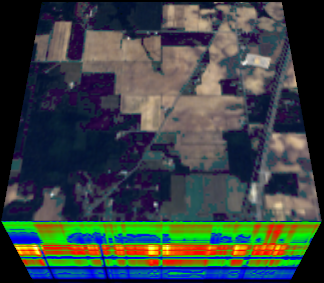
\includegraphics[width=8cm,height=8cm]{../india.png}};

\pic[shift={(0,0,0)}] at (0,0,0) 
    {Box={
        name=CNN_denoise_Conv0,
        caption= ,
        xlabel={{128, }},
        zlabel=145,
        fill=\ConvColor,
        height=32,
        width=2,
        depth=32
        }
    };

\pic[shift={ (0,0,0) }] at (CNN_denoise_Conv0-east) 
    {Box={
        name=BN0,
        caption= ,
        fill=\PoolColor,
        opacity=0.5,
        height=32,
        width=1,
        depth=32
        }
    };

\pic[shift={ (0,0,0) }] at (BN0-east) 
    {Box={
        name=RELU0,
        caption= ,
        fill=\mycolor,
        opacity=0.5,
        height=32,
        width=1,
        depth=32
        }
    };

\pic[shift={(1,0,0)}] at (RELU0-east) 
    {Box={
        name=CNN_denoise_Conv1,
        caption= ,
        xlabel={{128, }},
        zlabel=145,
        fill=\ConvColor,
        height=32,
        width=2,
        depth=32
        }
    };

\pic[shift={ (0,0,0) }] at (CNN_denoise_Conv1-east) 
    {Box={
        name=BN1,
        caption= ,
        fill=\PoolColor,
        opacity=0.5,
        height=32,
        width=1,
        depth=32
        }
    };

\pic[shift={ (0,0,0) }] at (BN1-east) 
    {Box={
        name=RELU1,
        caption= ,
        fill=\mycolor,
        opacity=0.5,
        height=32,
        width=1,
        depth=32
        }
    };

\draw [connection]  (RELU0-east)    -- node {\midarrow} (CNN_denoise_Conv1-west);

\pic[shift={ (2,0,0) }] at (RELU1-east) 
    {RightBandedBox={
        name=ccr_res_depth_conv0,
        caption= ,
        xlabel={{ 128, }},
        zlabel=145,
        fill={rgb:white,1;black,3},
        bandfill={rgb:white,1;black,2},
        opacity=0.1,
        height=32,
        width=1.0,
        depth=32
        }
    };

\pic[shift={(0,0,0)}] at (ccr_res_depth_conv0-east) 
    {Box={
        name=ccr_depth_conv0,
        caption= ,
        xlabel={{128, }},
        zlabel=145,
        fill=\ConvColor,
        height=32,
        width=1.0,
        depth=32
        }
    };

\pic[shift={ (0,0,0) }] at (ccr_depth_conv0-east) 
    {RightBandedBox={
        name=ccr_res_c_depth_conv0,
        caption= ,
        xlabel={{ 128, }},
        zlabel=145,
        fill={rgb:white,1;black,3},
        bandfill={rgb:white,1;black,2},
        opacity=0.1,
        height=32,
        width=1.0,
        depth=32
        }
    };

\pic[shift={(0,0,0)}] at (ccr_res_c_depth_conv0-east) 
    {Box={
        name=depth_conv0,
        caption= ,
        xlabel={{128, }},
        zlabel=145,
        fill=\ConvColor,
        height=32,
        width=1.0,
        depth=32
        }
    };

\pic[shift={ (0,0,0) }] at (depth_conv0-east) 
    {RightBandedBox={
        name=relu_depth_conv0,
        caption= ,
        xlabel={{ 1, 2 }},
        zlabel=145,
        fill=\mycolor,
        bandfill=\mycolor,
        height=32,
        width={ 1.0 , 1.0 },
        depth=32
        }
    };

\draw [connection]  (RELU1-east)    -- node {\midarrow} (relu_depth_conv0-west);

\pic[shift={(1.0,0,0)}] at (depth_conv0-east) 
    {Box={
        name=point_conv0,
        caption= ,
        xlabel={{" ","dummy"}},
        zlabel=128,
        fill=\mypoint,
        opacity=0.8,
        height=3,
        width=1.5,
        depth=25
        }
    };

\draw [connection]  (depth_conv0-east)    -- node {\midarrow} (point_conv0-west);

\pic[shift={ (1.0,0,0) }] at (point_conv0-east) 
    {Box={
        name=RELU2,
        caption= ,
        fill=\mycolor,
        opacity=0.5,
        height=32,
        width=1,
        depth=32
        }
    };

\pic[shift={ (0,0,0) }] at (RELU2-east) 
    {Box={
        name=BN2,
        caption= ,
        fill=\PoolColor,
        opacity=0.5,
        height=32,
        width=1,
        depth=32
        }
    };

\draw [connection]  (point_conv0-east)    -- node {\midarrow} (BN2-west);

\pic[shift={ (2,0,0) }] at (BN2-east) 
    {RightBandedBox={
        name=ccr_res_depth_conv1,
        caption= ,
        xlabel={{ 128, }},
        zlabel=145,
        fill={rgb:white,1;black,3},
        bandfill={rgb:white,1;black,2},
        opacity=0.1,
        height=32,
        width=1.0,
        depth=32
        }
    };

\pic[shift={(0,0,0)}] at (ccr_res_depth_conv1-east) 
    {Box={
        name=ccr_depth_conv1,
        caption= ,
        xlabel={{128, }},
        zlabel=145,
        fill=\ConvColor,
        height=32,
        width=1.0,
        depth=32
        }
    };

\pic[shift={ (0,0,0) }] at (ccr_depth_conv1-east) 
    {RightBandedBox={
        name=ccr_res_c_depth_conv1,
        caption= ,
        xlabel={{ 128, }},
        zlabel=145,
        fill={rgb:white,1;black,3},
        bandfill={rgb:white,1;black,2},
        opacity=0.1,
        height=32,
        width=1.0,
        depth=32
        }
    };

\pic[shift={(0,0,0)}] at (ccr_res_c_depth_conv1-east) 
    {Box={
        name=depth_conv1,
        caption= ,
        xlabel={{128, }},
        zlabel=145,
        fill=\ConvColor,
        height=32,
        width=1.0,
        depth=32
        }
    };

\pic[shift={ (0,0,0) }] at (depth_conv1-east) 
    {RightBandedBox={
        name=relu_depth_conv1,
        caption= ,
        xlabel={{ 1, 2 }},
        zlabel=145,
        fill=\mycolor,
        bandfill=\mycolor,
        height=32,
        width={ 1.0 , 1.0 },
        depth=32
        }
    };

\draw [connection]  (BN2-east)    -- node {\midarrow} (relu_depth_conv1-west);

\pic[shift={(1.0,0,0)}] at (depth_conv1-east) 
    {Box={
        name=point_conv1,
        caption= ,
        xlabel={{" ","dummy"}},
        zlabel=128,
        fill=\mypoint,
        opacity=0.8,
        height=3,
        width=1.5,
        depth=25
        }
    };

\draw [connection]  (depth_conv1-east)    -- node {\midarrow} (point_conv1-west);

\pic[shift={ (1.0,0,0) }] at (point_conv1-east) 
    {Box={
        name=RELU3,
        caption= ,
        fill=\mycolor,
        opacity=0.5,
        height=32,
        width=1,
        depth=32
        }
    };

\pic[shift={ (0,0,0) }] at (RELU3-east) 
    {Box={
        name=BN3,
        caption= ,
        fill=\PoolColor,
        opacity=0.5,
        height=32,
        width=1,
        depth=32
        }
    };

\draw [connection]  (point_conv1-east)    -- node {\midarrow} (BN3-west);

\pic[shift={ (2.0,0,0) }] at (BN3-east) 
    {RightBandedBox={
        name=CBAM,
        caption=CBAM,
        xlabel={{ 128, 128 }},
        zlabel=145,
        fill=\mycolor,
        bandfill=\mycolor,
        height=8,
        width={ 8 , 8 },
        depth=8
        }
    };

\draw [connection]  (BN3-east)    -- node {\midarrow} (CBAM-west);

\pic[shift={(2.0,0,0)}] at (CBAM-east) 
    {Box={
        name=soft1,
        caption=SOFT,
        xlabel={{" ","dummy"}},
        zlabel=16,
        fill=\SoftmaxColor,
        opacity=0.8,
        height=3,
        width=1.5,
        depth=25
        }
    };

\draw [connection]  (CBAM-east)    -- node {\midarrow} (soft1-west);

\pic[shift={(2.0,0,0)}] at (soft1-east) 
    {Ball={
        name=sum1,
        fill=\SumColor,
        opacity=0.6,
        radius=2.5,
        logo=$+$
        }
    };

\draw [connection]  (soft1-east)    -- node {\midarrow} (sum1-west);

\end{tikzpicture}
\end{document}
